\documentclass{article}
\usepackage{amsmath}
\usepackage{amssymb}
\usepackage{graphicx}
\usepackage{tikz}
\usepackage{pgfplots}
\usepackage{float}
\usepackage{subcaption}
\usepackage{geometry}

\geometry{a4paper, margin=1in}

% Define example environment
\newenvironment{example}[1]{
    \begin{trivlist}
    \item[\textbf{Example:}] #1
    \vspace{0.5em}
}{
    \end{trivlist}
    \vspace{1em}
}

\pgfplotsset{compat=1.18}
\usetikzlibrary{patterns,decorations.pathreplacing}

\title{Lecture 6 Examples}
\author{Signals and Systems Course}
\date{}

\begin{document}

\maketitle

\begin{example}[1. Finding an LTI System's Output Using its Impulse Response]
\textbf{Problem:}
Given LTI system responses:
\begin{itemize}
    \item $x_1[n] = \delta[n] + \delta[n-1] \rightarrow y_1[n] = \frac{1}{2}(\delta[n] + \delta[n-1] - \delta[n-2] - \delta[n-3])$
    \item $x_2[n] = \delta[n] - \delta[n-1] \rightarrow y_2[n] = \frac{1}{2}(\delta[n] - \delta[n-1] + \delta[n-2] - \delta[n-3])$
\end{itemize}

Find the output for $x[n] = \cos(\pi n)$.

\begin{figure}[H]
    \centering
    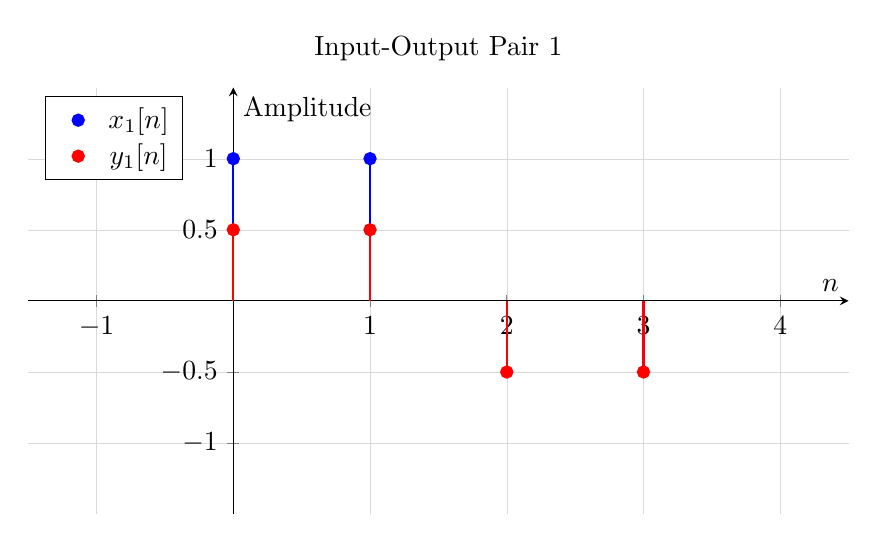
\begin{tikzpicture}
	\begin{axis}[
		width=12cm,
		height=7cm,
		axis lines=middle,
		xlabel={$n$},
		ylabel={Amplitude},
		title={Input-Output Pair 1},
		xmin=-1.5, xmax=4.5,
		ymin=-1.5, ymax=1.5,
		xtick={-1, 0, 1, 2, 3, 4},
		ytick={-1, -0.5, 0.5, 1},
		grid=major,
		grid style={line width=.1pt, draw=gray!30},
		legend style={
			at={(0.02,0.98)},
			anchor=north west,
		}
		]
		
		\addplot[blue, ycomb, thick, mark=*, mark size=2pt]
		coordinates {(0,1) (1,1)};
		\addlegendentry{$x_1[n]$};
		
		\addplot[red, ycomb, thick, mark=*, mark size=2pt]
		coordinates {(0,0.5) (1,0.5) (2,-0.5) (3,-0.5)};
		\addlegendentry{$y_1[n]$};
		
	\end{axis}
\end{tikzpicture}

\vspace{1cm}

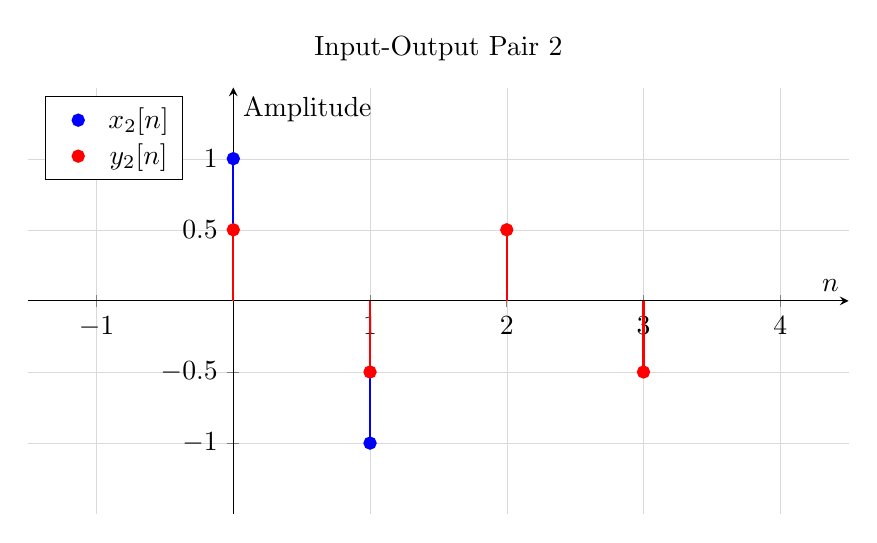
\begin{tikzpicture}
	\begin{axis}[
		width=12cm,
		height=7cm,
		axis lines=middle,
		xlabel={$n$},
		ylabel={Amplitude},
		title={Input-Output Pair 2},
		xmin=-1.5, xmax=4.5,
		ymin=-1.5, ymax=1.5,
		xtick={-1, 0, 1, 2, 3, 4},
		ytick={-1, -0.5, 0.5, 1},
		grid=major,
		grid style={line width=.1pt, draw=gray!30},
		legend style={
			at={(0.02,0.98)},
			anchor=north west,
		}
		]
		
		\addplot[blue, ycomb, thick, mark=*, mark size=2pt]
		coordinates {(0,1) (1,-1)};
		\addlegendentry{$x_2[n]$};
		
		\addplot[red, ycomb, thick, mark=*, mark size=2pt]
		coordinates {(0,0.5) (1,-0.5) (2,0.5) (3,-0.5)};
		\addlegendentry{$y_2[n]$};
		
	\end{axis}
\end{tikzpicture}

    \caption{The two known input-output pairs for the LTI system $S$.}
    \label{fig:io_pairs}
\end{figure}

\textbf{Solution:}

\textbf{Step 1: Find impulse response}
$$\delta[n] = \frac{1}{2}(x_1[n] + x_2[n])$$

$$h[n] = \frac{1}{2}(y_1[n] + y_2[n]) = \frac{1}{2}(\delta[n] - \delta[n-3])$$

\textbf{Step 2: Find output for $\cos(\pi n) = (-1)^n$}
$$y[n] = h[n] * (-1)^n = \frac{1}{2}(\delta[n] - \delta[n-3]) * (-1)^n$$

$$= \frac{1}{2}(-1)^n \sum_{k=-\infty}^{\infty} (\delta[k] - \delta[k-3]) (-1)^{-k}$$

$$= \frac{1}{2}(-1)^n [1 - (-1)] = (-1)^n$$

\textbf{Answer:} $y[n] = (-1)^n = \cos(\pi n)$
\end{example}

\vspace{0.5em}
\hrule
\vspace{0.5em}

\begin{example}[2. Inverse Systems and System Cascading]
\textbf{Problem:}
Given LTI systems:
\begin{itemize}
    \item System $S_1$: $y_1[n] = x[n-1]$ (delay of 1)
    \item System $S_2$: $y_2[n] = x[n+1]$ (advance of 1)
\end{itemize}

Find the overall system response when cascaded.

\textbf{Solution:}

\textbf{Impulse responses:}
\begin{align}
h_1[n] &= \delta[n-1] \\
h_2[n] &= \delta[n+1]
\end{align}

\textbf{Overall impulse response:}
$$h_{total}[n] = h_1[n] * h_2[n] = \delta[n-1] * \delta[n+1] = \delta[n]$$

\textbf{Answer:} $y[n] = x[n]$ (identity system)
\end{example}

\vspace{0.5em}
\hrule
\vspace{0.5em}

\begin{example}[3. First-Difference Filter as Inverse of Accumulator]
\textbf{Problem:}
Show that the first-difference filter is the inverse of the accumulator:
\begin{itemize}
    \item Accumulator: $y[n] = \sum_{k=-\infty}^{n} x[k]$
    \item First-difference filter: $y[n] = x[n] - x[n-1]$
\end{itemize}

\textbf{Solution:}

\textbf{Impulse responses:}
\begin{align}
h_{acc}[n] &= u[n] \\
h_{diff}[n] &= \delta[n] - \delta[n-1]
\end{align}

\textbf{Cascaded system:}
$$h_{total}[n] = u[n] * (\delta[n] - \delta[n-1]) = u[n] - u[n-1] = \delta[n]$$

\textbf{Answer:} The first-difference filter is the inverse of the accumulator.
\end{example}

\vspace{0.5em}
\hrule
\vspace{0.5em}

\begin{example}[4. Causality of LTI Systems]
\textbf{Problem:}
Determine which systems are causal:
\begin{enumerate}
    \item $h_1(t) = e^{-t} u(t)$
    \item $h_2(t) = e^{-|t|}$
    \item $h_3(t) = \delta(t+1)$
    \item $h_4(t) = e^{-t} u(-t)$
\end{enumerate}

\textbf{Solution:}

An LTI system is causal if $h(t) = 0$ for all $t < 0$.

\begin{itemize}
    \item System 1: $h_1(t) = 0$ for $t < 0$ → \textbf{Causal}
    \item System 2: $h_2(t) = e^{t} \neq 0$ for $t < 0$ → \textbf{Non-causal}
    \item System 3: $h_3(t) \neq 0$ at $t = -1 < 0$ → \textbf{Non-causal}
    \item System 4: $h_4(t) = e^{-t} \neq 0$ for $t < 0$ → \textbf{Non-causal}
\end{itemize}

\textbf{Answer:} Only System 1 is causal.
\end{example}

\vspace{0.5em}
\hrule
\vspace{0.5em}

\begin{example}[5. Finding Impulse Response from Integral Equation]
\textbf{Problem:}
Find the impulse response of the LTI system:
$$y(t) = \int_{-\infty}^{t} e^{-(t-\tau)} x(\tau) d\tau$$

\textbf{Solution:}

$$h(t) = \int_{-\infty}^{t} e^{-(t-\tau)} \delta(\tau) d\tau$$

For $t < 0$: $h(t) = 0$ (no overlap with $\delta(\tau)$)
For $t \geq 0$: $h(t) = e^{-t}$

\textbf{Answer:} $h(t) = e^{-t} u(t)$
\end{example}

\vspace{0.5em}
\hrule
\vspace{0.5em}

\begin{example}[6. BIBO Stability of LTI Systems]
\textbf{Problem:}
Determine BIBO stability of:
\begin{enumerate}
    \item $h_1[n] = a^n u[n]$, $|a| < 1$
    \item $h_2[n] = a^n u[n]$, $|a| \geq 1$
    \item $h_3(t) = e^{-at} u(t)$, $a > 0$
    \item $h_4(t) = e^{at} u(t)$, $a > 0$
\end{enumerate}

\textbf{Solution:}

\textbf{System 1:} $\sum_{n=0}^{\infty} |a|^n = \frac{1}{1-|a|} < \infty$ → \textbf{Stable}

\textbf{System 2:} $\sum_{n=0}^{\infty} |a|^n = \infty$ → \textbf{Not stable}

\textbf{System 3:} $\int_{0}^{\infty} e^{-at} dt = \frac{1}{a} < \infty$ → \textbf{Stable}

\textbf{System 4:} $\int_{0}^{\infty} e^{at} dt = \infty$ → \textbf{Not stable}

\textbf{Answer:} Systems 1 and 3 are BIBO stable; Systems 2 and 4 are not.
\end{example}

\vspace{0.5em}
\hrule
\vspace{0.5em}

\begin{example}[7. Autocorrelation of a One-Sided Exponential Signal]
\textbf{Problem:}
Find $R_{xx}(t)$ for $x(t) = 2e^{-3t}u(t)$ where $R_{xx}(t) = \int_{-\infty}^{\infty} x(\tau)x(\tau-t) d\tau$.

\begin{figure}[H]
    \centering
    \begin{tikzpicture}
	\begin{axis}[
		width=12cm,
		height=7cm,
		title={Exponential Signal $x(\tau) = A e^{-a\tau}u(\tau)$},
		xlabel={$\tau$},
		ylabel={$x(\tau)$},
		axis lines=middle,
		xmin=-1, xmax=4,
		ymin=0, ymax=2.2,
		xtick=\empty, ytick=\empty,
		extra x ticks={0.333},
		extra x tick labels={$\frac{1}{a}$},
		extra y ticks={0.736, 2},
		extra y tick labels={$Ae^{-1}$, $A$},
		grid=major,
		grid style={line width=.1pt, draw=gray!30},
		]
		\addplot[blue, very thick, domain=0:4, samples=200, no marks] {2*exp(-3*x)};
		\draw[blue, very thick] (axis cs:-1,0) -- (axis cs:0,0);
		\draw[dashed, gray] (axis cs:0.333,0) -- (axis cs:0.333, {2*exp(-1)});
		\draw[dashed, gray] (axis cs:0, {2*exp(-1)}) -- (axis cs:0.333, {2*exp(-1)});
	\end{axis}
\end{tikzpicture}
    \caption{The signal $x(\tau) = 2e^{-3\tau}u(\tau)$.}
\end{figure}

\textbf{Solution:}
\[ R_{xx}(t) = 4e^{3t} \int_{-\infty}^{\infty} e^{-6\tau}u(\tau)u(\tau-t) d\tau \]

\textbf{Case 1: $t \geq 0$} (overlap when $\tau \geq t$):
\[ R_{xx}(t) = 4e^{3t} \int_{t}^{\infty} e^{-6\tau} d\tau = \frac{2}{3}e^{-3t} \]

\textbf{Case 2: $t < 0$} (overlap when $\tau \geq 0$):
\[ R_{xx}(t) = 4e^{3t} \int_{0}^{\infty} e^{-6\tau} d\tau = \frac{2}{3}e^{3t} \]

\begin{figure}[H]
    \centering
    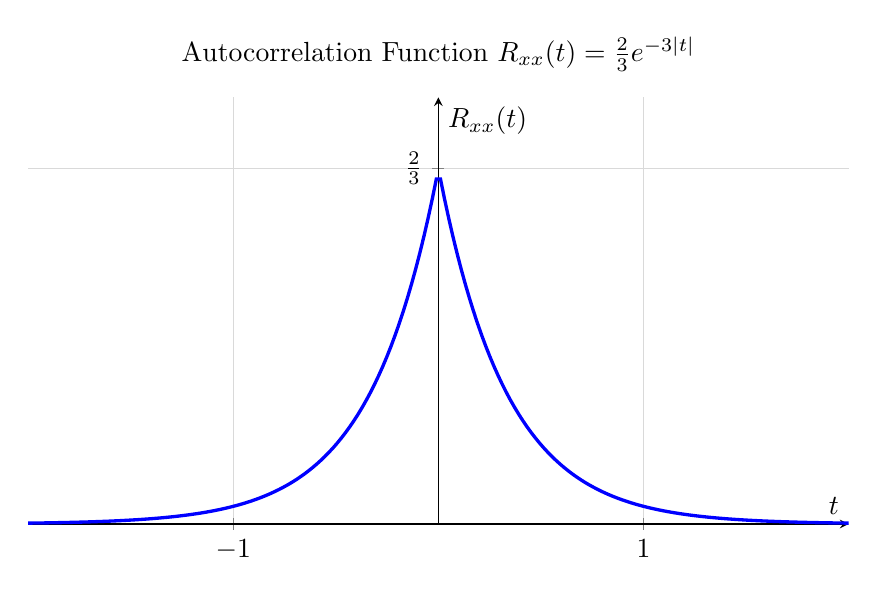
\begin{tikzpicture}
	\begin{axis}[
		width=12cm,
		height=7cm,
		title={Autocorrelation Function $R_{xx}(t) = \frac{2}{3}e^{-3|t|}$},
		xlabel={$t$},
		ylabel={$R_{xx}(t)$},
		axis lines=middle,
		xmin=-2, xmax=2,
		ymin=0, ymax=0.8,
		xtick={-1, 1},
		ytick={0.667},
		yticklabels={$\frac{2}{3}$},
		grid=major,
		grid style={line width=.1pt, draw=gray!30},
		]
		\addplot[blue, very thick, domain=-2:2, samples=200, no marks] {(2/3)*exp(-3*abs(x))};
	\end{axis}
\end{tikzpicture}
    \caption{The resulting autocorrelation function is a symmetric, two-sided exponential, which is maximal at $t=0$.}
\end{figure}

\textbf{Answer:} $R_{xx}(t) = \frac{2}{3}e^{-3|t|}$
\end{example}

\vspace{0.5em}
\hrule
\vspace{0.5em}

\begin{example}[8. Cross-Correlation of Two Rectangular Pulses]
\textbf{Problem:}
Given two continuous-time rectangular pulse signals, $x(t)$ and $y(t)$, defined as:
\begin{itemize}
    \item $x(t) = u(t) - u(t-1)$
    \item $y(t) = u(t - 3/2) - u(t - 5/2)$
\end{itemize}
Find the cross-correlation functions $R_{yx}(t)$ and $R_{xy}(t)$. These are defined by the integrals:
\[ R_{yx}(t) = \int_{-\infty}^{\infty} y(\tau)x(\tau-t) d\tau \]
\[ R_{xy}(t) = \int_{-\infty}^{\infty} x(\tau)y(\tau-t) d\tau \]

\begin{figure}[H]
    \centering
    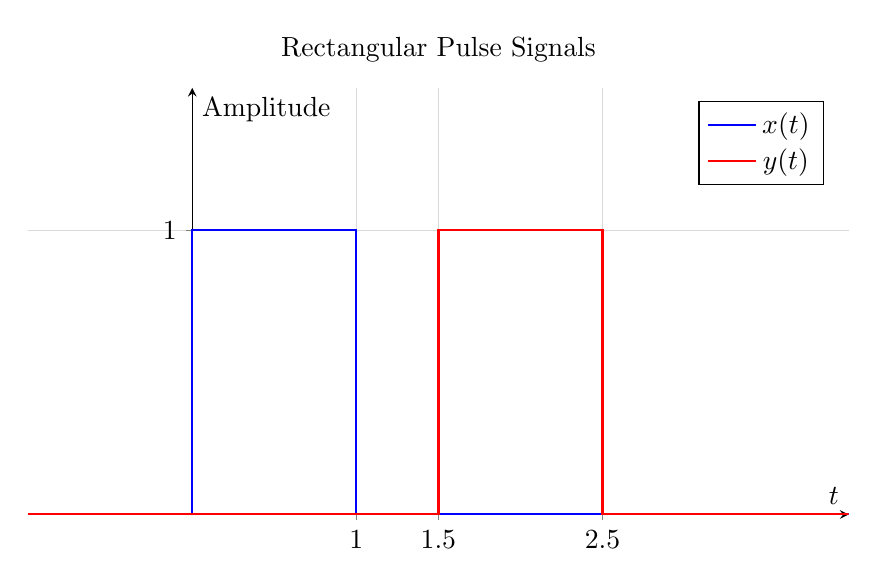
\begin{tikzpicture}
	\begin{axis}[
		width=12cm,
		height=7cm,
		title={Rectangular Pulse Signals},
		xlabel={$t$},
		ylabel={Amplitude},
		axis lines=middle,
		xmin=-1, xmax=4,
		ymin=0, ymax=1.5,
		xtick={0,1,1.5,2.5},
		ytick={1},
		grid=major,
		grid style={line width=.1pt, draw=gray!30},
		legend pos=north east,
		]
		% x(t)
		\addplot+[blue, thick, mark=none] coordinates {
			(-1,0) (0,0) (0,1) (1,1) (1,0) (4,0)
		};
		\addlegendentry{$x(t)$}
		
		% y(t)
		\addplot+[red, thick, mark=none] coordinates {
			(-1,0) (1.5,0) (1.5,1) (2.5,1) (2.5,0) (4,0)
		};
		\addlegendentry{$y(t)$}
	\end{axis}
\end{tikzpicture}
    \caption{The two rectangular pulse signals $x(t)$ and $y(t)$.}
\end{figure}

\textbf{Solution:}
The cross-correlation integral represents the area of overlap between one signal and a time-shifted version of the other. Since both signals are pulses of height 1, the value of the integral is simply the length of the interval over which they overlap.

\textbf{Calculation of $R_{xy}(t)$:}
We need to find the overlap between $x(\tau)$ (which exists for $0 \leq \tau \leq 1$) and $y(\tau-t)$ (which exists for $3/2 \leq \tau-t \leq 5/2$, or $3/2+t \leq \tau \leq 5/2+t$).

The overlap occurs when both conditions are satisfied:
\begin{itemize}
    \item $0 \leq \tau \leq 1$ (from $x(\tau)$)
    \item $3/2+t \leq \tau \leq 5/2+t$ (from $y(\tau-t)$)
\end{itemize}

This gives us different cases based on the value of $t$:

\textbf{Case 1: $t \leq -5/2$} - No overlap, $R_{xy}(t) = 0$

\textbf{Case 2: $-5/2 < t \leq -3/2$} - Partial overlap
The overlap interval is $[0, 5/2+t]$, so:
\[ R_{xy}(t) = 5/2 + t \]

\textbf{Case 3: $-3/2 < t \leq -1/2$} - Partial overlap
The overlap interval is $[3/2+t, 1]$, so:
\[ R_{xy}(t) = 1 - (3/2+t) = -1/2 - t \]

\textbf{Case 4: $t \geq -1/2$} - No overlap, $R_{xy}(t) = 0$

\begin{figure}[H]
    \centering
    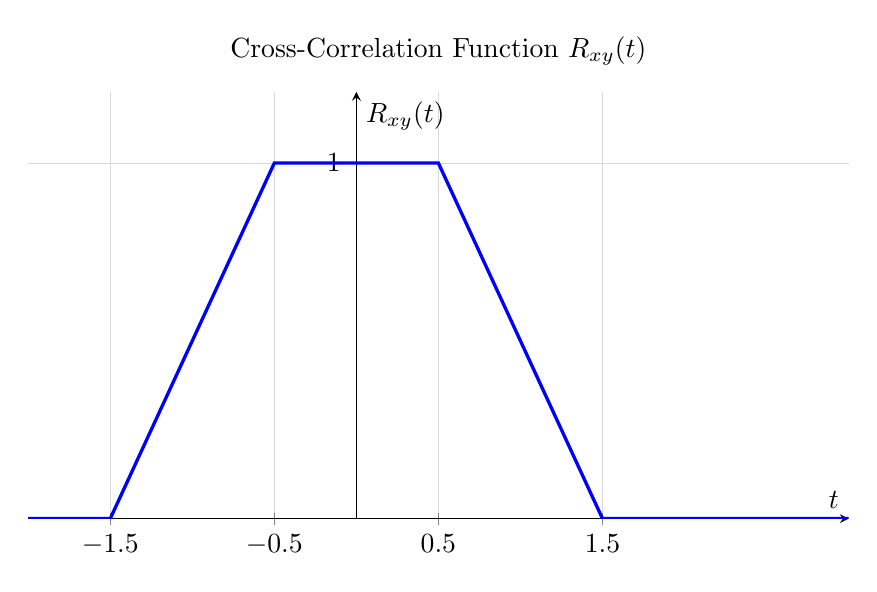
\begin{tikzpicture}
	\begin{axis}[
		width=12cm,
		height=7cm,
		title={Cross-Correlation Function $R_{xy}(t)$},
		xlabel={$t$},
		ylabel={$R_{xy}(t)$},
		axis lines=middle,
		xmin=-2, xmax=3,
		ymin=0, ymax=1.2,
		xtick={-1.5, -0.5, 0.5, 1.5},
		ytick={1},
		grid=major,
		grid style={line width=.1pt, draw=gray!30},
		]
		\draw[blue, very thick]
		(axis cs:-2,0) -- (axis cs:-1.5,0) -- (axis cs:-0.5,1)
		-- (axis cs:0.5,1) -- (axis cs:1.5,0) -- (axis cs:3,0);
	\end{axis}
\end{tikzpicture}
    \caption{The two cross-correlation functions.}
\end{figure}

\textbf{Answer:} The cross-correlation functions are:
\[
R_{xy}(t) = 
\begin{cases}
0 & t \leq -5/2 \\
5/2 + t & -5/2 < t \leq -3/2 \\
-1/2 - t & -3/2 < t < -1/2 \\
0 & t \geq -1/2
\end{cases}
\]

And by the property of cross-correlation: $R_{yx}(t) = R_{xy}(-t)$
\end{example}

\vspace{0.5em}
\hrule
\vspace{0.5em}

\begin{example}[9. Autocorrelation of a Discrete-Time Exponential Sequence]
\textbf{Problem:}
For the discrete-time signal $x[n]$, defined as a one-sided exponential sequence:
\[ x[n] = \left(\frac{1}{2}\right)^n u[n] \]
Find its autocorrelation function, $R_{xx}[n]$, which is defined by the summation:
\[ R_{xx}[n] = \sum_{k=-\infty}^{\infty} x[k] x[k-n] \]

\begin{figure}[H]
    \centering
    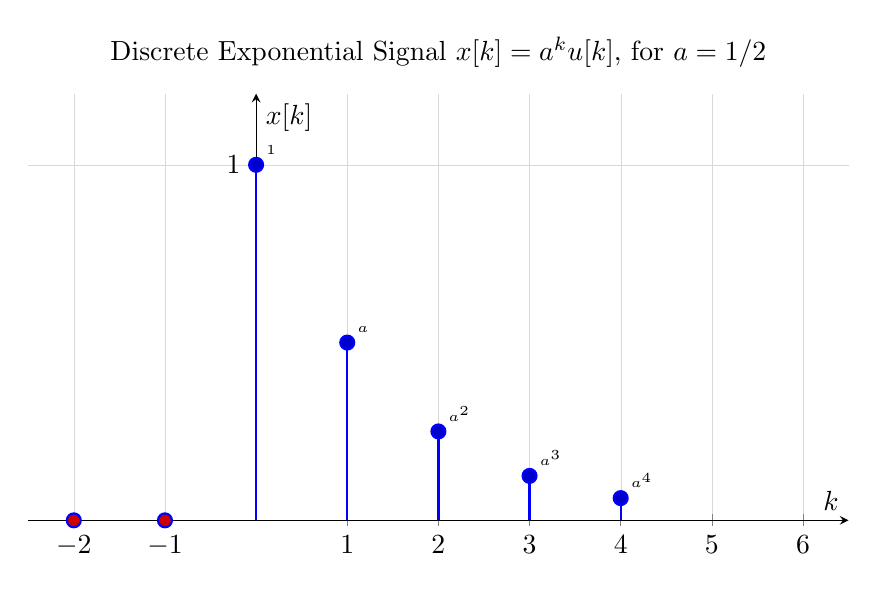
\begin{tikzpicture}
	\pgfplotsset{impulse/.style={ycomb,blue,thick,mark=*,mark size=2.5pt}}
	\begin{axis}[
		width=12cm,
		height=7cm,
		title={Discrete Exponential Signal $x[k] = a^k u[k]$, for $a=1/2$},
		xlabel={$k$},
		ylabel={$x[k]$},
		axis lines=middle,
		xmin=-2.5, xmax=6.5,
		ymin=0, ymax=1.2,
		xtick={-2,-1,0,1,2,3,4,5,6},
		ytick={1},
		grid=major,
		grid style={line width=.1pt, draw=gray!30},
		]
		\addplot+[impulse,nodes near coords,point meta=explicit symbolic,
		every node near coord/.style={anchor=south west,font=\tiny,text=black}] 
		table [meta=label] {
			x y label
			0 1 {$1$}
			1 0.5 {$a$}
			2 0.25 {$a^2$}
			3 0.125 {$a^3$}
			4 0.0625 {$a^4$}
		};
		\addplot+[impulse] coordinates {(-2,0)(-1,0)};
	\end{axis}
\end{tikzpicture}
    \caption{The signal $x[k] = (1/2)^k u[k]$.}
\end{figure}

\textbf{Solution:}
We substitute the definition of $x[n]$ into the autocorrelation summation:
\[ R_{xx}[n] = \sum_{k=-\infty}^{\infty} \left(\frac{1}{2}\right)^k u[k] \left(\frac{1}{2}\right)^{k-n} u[k-n] \]

Simplifying:
\[ R_{xx}[n] = \left(\frac{1}{2}\right)^{-n} \sum_{k=-\infty}^{\infty} \left(\frac{1}{2}\right)^{2k} u[k] u[k-n] \]

The product $u[k]u[k-n]$ is non-zero only when both step functions are 1, which occurs when $k \geq 0$ and $k \geq n$. This gives us two cases:

\textbf{Case 1: $n \geq 0$}
For $n \geq 0$, both conditions are satisfied when $k \geq n$. The summation becomes:
\[ R_{xx}[n] = \left(\frac{1}{2}\right)^{-n} \sum_{k=n}^{\infty} \left(\frac{1}{2}\right)^{2k} = \left(\frac{1}{2}\right)^{-n} \left(\frac{1}{2}\right)^{2n} \sum_{k=0}^{\infty} \left(\frac{1}{4}\right)^k \]

Using the geometric series formula:
\[ R_{xx}[n] = \left(\frac{1}{2}\right)^n \cdot \frac{1}{1-1/4} = \left(\frac{1}{2}\right)^n \cdot \frac{4}{3} = \frac{4}{3} \left(\frac{1}{2}\right)^n \]

\textbf{Case 2: $n < 0$}
For $n < 0$, both conditions are satisfied when $k \geq 0$. The summation becomes:
\[ R_{xx}[n] = \left(\frac{1}{2}\right)^{-n} \sum_{k=0}^{\infty} \left(\frac{1}{2}\right)^{2k} = \left(\frac{1}{2}\right)^{-n} \cdot \frac{1}{1-1/4} = \frac{4}{3} \left(\frac{1}{2}\right)^{-n} \]

\begin{figure}[H]
    \centering
    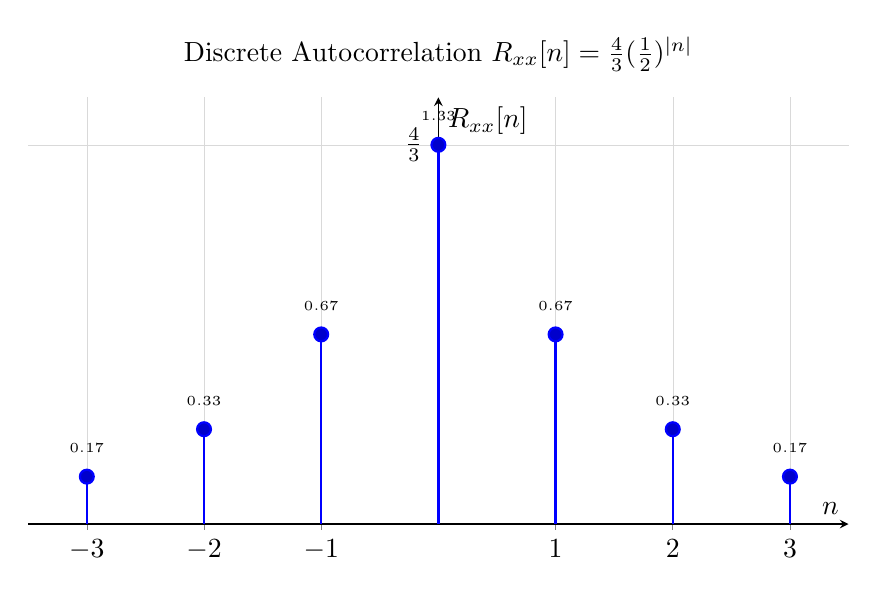
\begin{tikzpicture}
	\pgfplotsset{impulse/.style={ycomb,blue,thick,mark=*,mark size=2.5pt}}
	\begin{axis}[
		width=12cm,
		height=7cm,
		title={Discrete Autocorrelation $R_{xx}[n] = \frac{4}{3}(\frac{1}{2})^{|n|}$},
		xlabel={$n$},
		ylabel={$R_{xx}[n]$},
		axis lines=middle,
		xmin=-3.5, xmax=3.5,
		ymin=0, ymax=1.5,
		xtick={-3,-2,-1,0,1,2,3},
		ytick={1.333},
		yticklabels={$\frac{4}{3}$},
		grid=major,
		grid style={line width=.1pt, draw=gray!30},
		]
		\addplot+[impulse, samples at={-3,...,3}, nodes near coords,
		every node near coord/.style={font=\tiny, text=black,
			yshift=5pt, anchor=south},] {(4/3)*(1/2)^abs(x)};
	\end{axis}
\end{tikzpicture}
    \caption{The resulting autocorrelation function is a symmetric, two-sided exponential sequence.}
\end{figure}

\textbf{Answer:} The autocorrelation function is:
\[
R_{xx}[n] = 
\begin{cases}
\frac{4}{3} \left(\frac{1}{2}\right)^n & n \geq 0 \\
\frac{4}{3} \left(\frac{1}{2}\right)^{-n} & n < 0
\end{cases}
= \frac{4}{3} \left(\frac{1}{2}\right)^{|n|}
\]
\end{example}

\vspace{0.5em}
\hrule
\vspace{0.5em}

\begin{example}[10. Cross-Correlation of Two Discrete-Time Signals]
\textbf{Problem:}
Compute the cross-correlation $R_{xy}[n]$ for the two discrete-time signals $x[n]$ and $y[n]$:

The signals can be expressed mathematically as:
\[
x[n] = 2\delta[n+1] + 4\delta[n] - 3\delta[n-1]
\]
\[
y[n] = -3\delta[n+1] + \delta[n-1]
\]
where $\delta[n]$ is the unit impulse function. The non-zero values are:
\begin{itemize}
    \item $x[-1]=2$, $x[0]=4$, $x[1]=-3$
    \item $y[-1]=-3$, $y[0]=0$, $y[1]=1$
\end{itemize}

\begin{figure}[H]
    \centering
    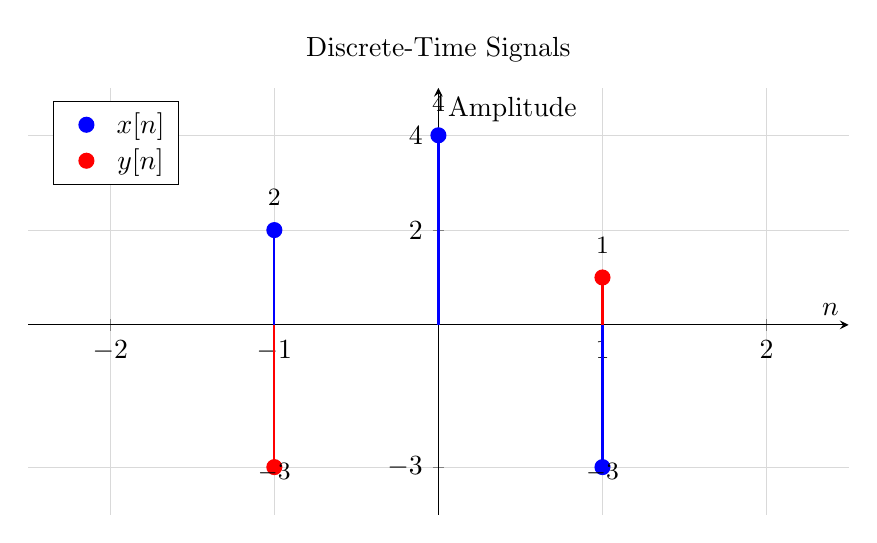
\begin{tikzpicture}
	\pgfplotsset{impulse/.style={ycomb,thick,mark=*,mark size=2.5pt}}
	\begin{axis}[
		width=12cm,
		height=7cm,
		title={Discrete-Time Signals},
		xlabel={$n$},
		ylabel={Amplitude},
		axis lines=middle,
		xmin=-2.5, xmax=2.5,
		ymin=-4, ymax=5,
		xtick={-2,-1,0,1,2},
		ytick={-3, 2, 4},
		grid=major,
		grid style={line width=.1pt, draw=gray!30},
		legend pos=north west,
		]
		\addplot[impulse, blue, nodes near coords,
		every node near coord/.style={yshift=5pt,font=\small,text=black}] 
		coordinates {(-1,2) (0,4) (1,-3)};
		\addlegendentry{$x[n]$};
		
		\addplot[impulse, red, nodes near coords,
		every node near coord/.style={yshift=5pt,font=\small,text=black}] 
		coordinates {(-1,-3) (1,1)};
		\addlegendentry{$y[n]$};
	\end{axis}
\end{tikzpicture}
    \caption{The two discrete-time signals $x[n]$ and $y[n]$.}
\end{figure}

\textbf{Solution:}
The cross-correlation is defined as:
\[ R_{xy}[n] = \sum_{k=-\infty}^{\infty} x[k] y[k-n] \]

Since both signals have finite support, we only need to consider the non-zero terms. Let's compute $R_{xy}[n]$ for different values of $n$:

\textbf{For $n = -2$:}
\[ R_{xy}[-2] = \sum_{k} x[k] y[k+2] = x[-1]y[1] + x[0]y[2] + x[1]y[3] = 2 \cdot 1 + 4 \cdot 0 + (-3) \cdot 0 = 2 \]

\textbf{For $n = -1$:}
\[ R_{xy}[-1] = \sum_{k} x[k] y[k+1] = x[-1]y[0] + x[0]y[1] + x[1]y[2] = 2 \cdot 0 + 4 \cdot 1 + (-3) \cdot 0 = 4 \]

\textbf{For $n = 0$:}
\[ R_{xy}[0] = \sum_{k} x[k] y[k] = x[-1]y[-1] + x[0]y[0] + x[1]y[1] = 2 \cdot (-3) + 4 \cdot 0 + (-3) \cdot 1 = -9 \]

\textbf{For $n = 1$:}
\[ R_{xy}[1] = \sum_{k} x[k] y[k-1] = x[-1]y[-2] + x[0]y[-1] + x[1]y[0] = 2 \cdot 0 + 4 \cdot (-3) + (-3) \cdot 0 = -12 \]

\textbf{For $n = 2$:}
\[ R_{xy}[2] = \sum_{k} x[k] y[k-2] = x[-1]y[-3] + x[0]y[-2] + x[1]y[-1] = 2 \cdot 0 + 4 \cdot 0 + (-3) \cdot (-3) = 9 \]

For all other values of $n$, $R_{xy}[n] = 0$.

\begin{figure}[H]
    \centering
    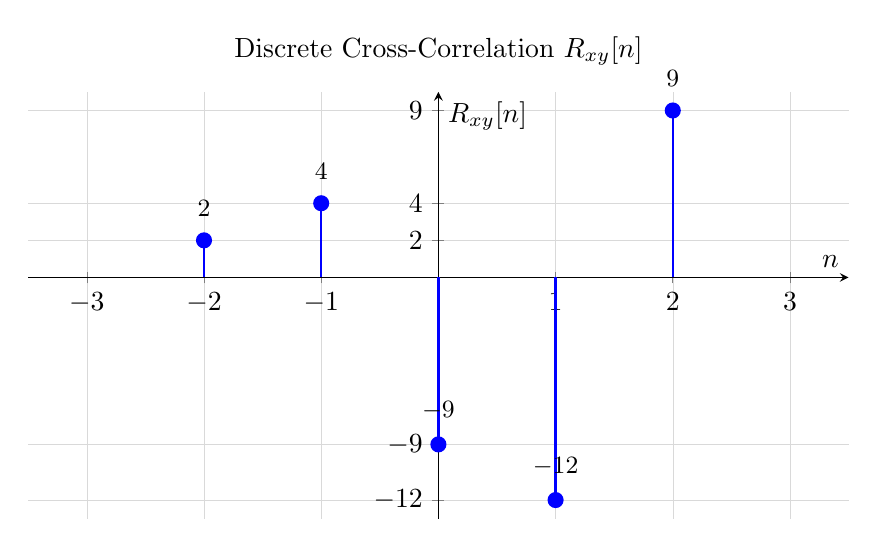
\begin{tikzpicture}
	\pgfplotsset{impulse/.style={ycomb,blue,thick,mark=*,mark size=2.5pt}}
	\begin{axis}[
		width=12cm,
		height=7cm,
		title={Discrete Cross-Correlation $R_{xy}[n]$},
		xlabel={$n$},
		ylabel={$R_{xy}[n]$},
		axis lines=middle,
		xmin=-3.5, xmax=3.5,
		ymin=-13, ymax=10,
		xtick={-3,-2,-1,0,1,2,3},
		ytick={-12, -9, 2, 4, 9},
		grid=major,
		grid style={line width=.1pt, draw=gray!30},
		]
		\addplot[impulse, nodes near coords,
		every node near coord/.style={font=\small,text=black,
			yshift=5pt, anchor=south}]
		coordinates {(-2,2) (-1,4) (0,-9) (1,-12) (2,9)};
	\end{axis}
\end{tikzpicture}
    \caption{The cross-correlation function $R_{xy}[n]$.}
\end{figure}

\textbf{Answer:} The cross-correlation function is:
\[
R_{xy}[n] = 
\begin{cases}
2 & n = -2 \\
4 & n = -1 \\
-9 & n = 0 \\
-12 & n = 1 \\
9 & n = 2 \\
0 & \text{otherwise}
\end{cases}
\]
\end{example}

\vspace{0.5em}
\hrule
\vspace{0.5em}

\begin{example}[11. Autocorrelation of a Continuous-Time Rectangular Pulse]
\textbf{Problem:}
Given the continuous-time rectangular pulse signal:
\[ x(t) = u(t) - u(t-1) \]
where $u(t)$ is the continuous-time unit step function.

Find the autocorrelation function of this signal, denoted by $R_{xx}(t)$, which is defined by the integral:
\[ R_{xx}(t) = \int_{-\infty}^{\infty} x(\tau)x(\tau - t) \,d\tau \]

\begin{figure}[H]
    \centering
    \begin{tikzpicture}
	\begin{axis}[
		width=12cm,
		height=7cm,
		title={Rectangular Pulse $x(t) = u(t) - u(t-T)$},
		xlabel={$t$},
		ylabel={$x(t)$},
		axis lines=middle,
		xmin=-1, xmax=2.5,
		ymin=0, ymax=1.5,
		xtick={1},
		xticklabels={$T$},
		ytick={1},
		yticklabels={$A$},
		grid=major,
		grid style={line width=.1pt, draw=gray!30},
		]
		\draw[blue, very thick]
		(axis cs:-1,0) -- (axis cs:0,0) -- (axis cs:0,1) 
		-- (axis cs:1,1) -- (axis cs:1,0) -- (axis cs:2.5,0);
	\end{axis}
\end{tikzpicture}
    \caption{The rectangular pulse signal $x(t) = u(t) - u(t-1)$.}
\end{figure}

\textbf{Solution:}
The autocorrelation function $R_{xx}(t)$ can be interpreted as the convolution of $x(t)$ with its time-reversed version, $x(-t)$. For a real-valued signal like this one, it measures the area of overlap between the signal $x(\tau)$ and a version of itself, $x(\tau-t)$, that has been shifted by an amount $t$.

\textbf{Intuitive Approach: Graphical "Slide and Overlap"}
We can visualize the calculation by fixing the signal $x(\tau)$ in place and "sliding" a shifted copy, $x(\tau-t)$, across it. The value of the autocorrelation $R_{xx}(t)$ for any given shift $t$ is simply the area of the overlapping region between the two pulses.

\begin{itemize}
    \item The fixed pulse $x(\tau)$ occupies the interval $[0, 1]$.
    \item The sliding pulse $x(\tau-t)$ occupies the interval $[t, 1+t]$.
    \item The autocorrelation $R_{xx}(t)$ will be the area of the intersection of these two intervals.
\end{itemize}

This graphical method shows that the overlap will only occur for shifts between $t=-1$ and $t=1$. Outside this range, the pulses do not overlap, and the autocorrelation is zero. The overlap area will be maximum (equal to 1) at $t=0$ and will decrease linearly to zero as $t$ approaches $-1$ or $1$. This predicts a triangular shape for the result.

\textbf{Mathematical Calculation}
We need to evaluate the integral:
\[ R_{xx}(t) = \int_{-\infty}^{\infty} x(\tau)x(\tau-t) \,d\tau \]

Since $x(\tau) = 1$ for $0 \leq \tau \leq 1$ and $0$ otherwise, and $x(\tau-t) = 1$ for $t \leq \tau \leq 1+t$ and $0$ otherwise, the integrand is non-zero only when both conditions are satisfied.

\textbf{Case 1: $t \leq -1$}
No overlap occurs, so $R_{xx}(t) = 0$.

\textbf{Case 2: $-1 < t \leq 0$}
The overlap interval is $[0, 1+t]$, so:
\[ R_{xx}(t) = \int_{0}^{1+t} 1 \cdot 1 \,d\tau = 1 + t \]

\textbf{Case 3: $0 < t \leq 1$}
The overlap interval is $[t, 1]$, so:
\[ R_{xx}(t) = \int_{t}^{1} 1 \cdot 1 \,d\tau = 1 - t \]

\textbf{Case 4: $t > 1$}
No overlap occurs, so $R_{xx}(t) = 0$.

\begin{figure}[H]
    \centering
    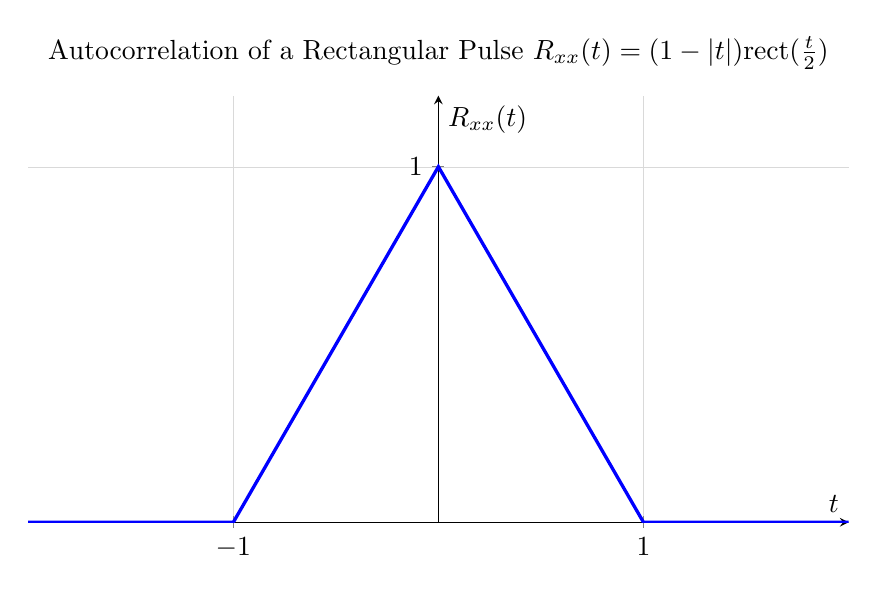
\begin{tikzpicture}
	\begin{axis}[
		width=12cm,
		height=7cm,
		title={Autocorrelation of a Rectangular Pulse $R_{xx}(t) = (1-|t|) \text{rect}(\frac{t}{2})$},
		xlabel={$t$},
		ylabel={$R_{xx}(t)$},
		axis lines=middle,
		xmin=-2, xmax=2,
		ymin=0, ymax=1.2,
		xtick={-1, 1},
		ytick={1},
		grid=major,
		grid style={line width=.1pt, draw=gray!30},
		]
		\draw[blue, very thick]
		(axis cs:-2,0) -- (axis cs:-1,0) -- (axis cs:0,1) 
		-- (axis cs:1,0) -- (axis cs:2,0);
	\end{axis}
\end{tikzpicture}
    \caption{The resulting triangular autocorrelation function $R_{xx}(t)$.}
\end{figure}

\textbf{Answer:} The autocorrelation function is:
\[
R_{xx}(t) = 
\begin{cases}
0 & t \leq -1 \\
1 + t & -1 < t \leq 0 \\
1 - t & 0 < t \leq 1 \\
0 & t > 1
\end{cases}
= \max(0, 1 - |t|)
\]
\end{example}

\vspace{0.5em}
\hrule
\vspace{0.5em}

\begin{example}[12. Fundamental Properties of Correlation Functions]
\textbf{Problem:}
This problem consists of two independent proofs regarding correlation functions.

\begin{enumerate}
    \item \textbf{Autocorrelation Maximum Property:} Show that for any real-valued energy signal $x(t)$, its autocorrelation function, $R_{xx}(t)$, satisfies the following inequality for all $t$:
    \[ R_{xx}(0) \ge R_{xx}(t) \]
    
    \item \textbf{Correlation-Convolution Relationship:} Show that the cross-correlation of two real-valued signals, $x(t)$ and $y(t)$, can be expressed as the convolution of one signal with the time-reversed version of the other:
    \[ R_{xy}(t) = x(t) * y(-t) \]
\end{enumerate}

\textbf{Solution:}
We will prove each statement step-by-step.

\textbf{Proof 1: Autocorrelation Maximum at the Origin}
This property states that a signal is always most similar to itself when there is no time shift.

\textbf{Intuitive Approach:}
The autocorrelation function, $R_{xx}(t) = \int_{-\infty}^{\infty} x(\tau)x(\tau-t) \,d\tau$, measures the area of the product of a signal and a time-shifted version of itself. At $t=0$, the function is $R_{xx}(0) = \int_{-\infty}^{\infty} x^2(\tau) \,d\tau$, which is the total energy of the signal. Since $x^2(\tau)$ is always non-negative, this integral represents the maximum possible overlap area. Any shift ($t \neq 0$) is likely to reduce the alignment between positive and negative parts of the signal, thus reducing the value of the integral.

\textbf{Mathematical Proof:}
Consider the integral:
\[ \int_{-\infty}^{\infty} [x(\tau) - x(\tau-t)]^2 \,d\tau \geq 0 \]

Expanding the square:
\[ \int_{-\infty}^{\infty} [x^2(\tau) - 2x(\tau)x(\tau-t) + x^2(\tau-t)] \,d\tau \geq 0 \]

Using the linearity of integration, we can split this into three separate integrals:
\[ \int_{-\infty}^{\infty} x^2(\tau) \,d\tau - 2\int_{-\infty}^{\infty} x(\tau)x(\tau-t) \,d\tau + \int_{-\infty}^{\infty} x^2(\tau-t) \,d\tau \geq 0 \]

We now identify each of these terms based on the definition of autocorrelation:
\begin{itemize}
    \item $\int_{-\infty}^{\infty} x^2(\tau) \,d\tau = R_{xx}(0)$ (This is the autocorrelation at zero lag, i.e., the signal's energy).
    \item $\int_{-\infty}^{\infty} x(\tau)x(\tau-t) \,d\tau = R_{xx}(t)$ (This is the definition of the autocorrelation function).
    \item $\int_{-\infty}^{\infty} x^2(\tau-t) \,d\tau = R_{xx}(0)$ (The energy of a signal is invariant to a time shift).
\end{itemize}

Substituting these into our inequality:
\[ R_{xx}(0) - 2R_{xx}(t) + R_{xx}(0) \geq 0 \]
\[ 2R_{xx}(0) - 2R_{xx}(t) \geq 0 \]
\[ R_{xx}(0) - R_{xx}(t) \geq 0 \]

Therefore:
\[ \boxed{R_{xx}(0) \ge R_{xx}(t)} \]

\textbf{Proof 2: Relationship Between Correlation and Convolution}
We need to show that $R_{xy}(t) = x(t) * y(-t)$.

Starting with the definition of cross-correlation:
\[ R_{xy}(t) = \int_{-\infty}^{\infty} x(\tau) y(\tau-t) \,d\tau \]

Let's make a substitution: let $u = \tau - t$, so $\tau = u + t$ and $d\tau = du$. When $\tau \to -\infty$, $u \to -\infty$, and when $\tau \to \infty$, $u \to \infty$.

\[ R_{xy}(t) = \int_{-\infty}^{\infty} x(u+t) y(u) \,du \]

Now let's make another substitution: let $v = -u$, so $u = -v$ and $du = -dv$. When $u \to -\infty$, $v \to \infty$, and when $u \to \infty$, $v \to -\infty$.

\[ R_{xy}(t) = \int_{\infty}^{-\infty} x(-v+t) y(-v) (-dv) = \int_{-\infty}^{\infty} x(t-v) y(-v) \,dv \]

This is exactly the definition of convolution between $x(t)$ and $y(-t)$:
\[ R_{xy}(t) = x(t) * y(-t) \]

Therefore:
\[ \boxed{R_{xy}(t) = x(t) * y(-t)} \]

\textbf{Answer:} Both properties have been proven:
\begin{enumerate}
    \item The autocorrelation function reaches its maximum at zero lag: $R_{xx}(0) \ge R_{xx}(t)$ for all $t$.
    \item The cross-correlation can be expressed as a convolution: $R_{xy}(t) = x(t) * y(-t)$.
\end{enumerate}
\end{example}

\end{document}